%-----------------------------------------------------------------------------------------------------------------------------------------------%
%	The MIT License (MIT)
%
%	Copyright (c) 2015 Jan Küster
%
%	Permission is hereby granted, free of charge, to any person obtaining a copy
%	of this software and associated documentation files (the "Software"), to deal
%	in the Software without restriction, including without limitation the rights
%	to use, copy, modify, merge, publish, distribute, sublicense, and/or sell
%	copies of the Software, and to permit persons to whom the Software is
%	furnished to do so, subject to the following conditions:
%
%	THE SOFTWARE IS PROVIDED "AS IS", WITHOUT WARRANTY OF ANY KIND, EXPRESS OR
%	IMPLIED, INCLUDING BUT NOT LIMITED TO THE WARRANTIES OF MERCHANTABILITY,
%	FITNESS FOR A PARTICULAR PURPOSE AND NONINFRINGEMENT. IN NO EVENT SHALL THE
%	AUTHORS OR COPYRIGHT HOLDERS BE LIABLE FOR ANY CLAIM, DAMAGES OR OTHER
%	LIABILITY, WHETHER IN AN ACTION OF CONTRACT, TORT OR OTHERWISE, ARISING FROM,
%	OUT OF OR IN CONNECTION WITH THE SOFTWARE OR THE USE OR OTHER DEALINGS IN
%	THE SOFTWARE.
%
%
%-----------------------------------------------------------------------------------------------------------------------------------------------%

%============================================================================%
%	DOCUMENT DEFINITION
%============================================================================%

%we use article class because we want to fully customize the page and dont use a cv template
\documentclass[10pt,letterpaper]{article}



%	ENCODING

%we use utf8 since we want to build from any machine
\usepackage[utf8]{inputenc}



%	LOGIC

% provides \isempty test
\usepackage{xifthen}



%	FONT

% some tex-live fonts - choose your own

%\usepackage[defaultsans]{droidsans}
%\usepackage[default]{comfortaa}
%\usepackage{cmbright}
%\usepackage[default]{raleway}
%\usepackage{fetamont}
%\usepackage[default]{gillius}
%\usepackage[light,math]{iwona}
% \usepackage[thin]{roboto}

% set font default
\renewcommand*\familydefault{\sfdefault}
\usepackage[T1]{fontenc}

% more font size definitions
\usepackage{moresize}



%	PAGE LAYOUT  DEFINITIONS

%debug page outer frames
%\usepackage{showframe}

%define page styles using geometry
\usepackage[letterpaper]{geometry}

% for example, change the margins to 2 inches all round
\geometry{top=1.75cm, bottom=-.6cm, left=1.5cm, right=1.5cm}

%use customized header
\usepackage{fancyhdr}
\pagestyle{fancy}

%less space between header and content
\setlength{\headheight}{-5pt}

%customize entries left, center and right
\lhead{}
\chead{
  \textcolor{txtcol}{\textbf{Consultant and Software Engineer}} \textcolor{sectcol}{$\oplus$}
  \textcolor{txtcol}{\textbf{Roanoke, Virgina}} \textcolor{sectcol}{$\oplus$}
  \textcolor{txtcol}{\textbf{dconner@xel.io}} \textcolor{sectcol}{$\oplus$}
  \textcolor{txtcol}{\textbf{+1 (540) 761-1257}}
}
\rhead{}

% it's unclear how hyphenation affects keyword detection. turn it off
\usepackage[none]{hyphenat}

% hyphenat adds too much space. a global \raggedright isn't working. it looks
% terrible in sections where it does (throws off blocks).
% sooo... manually balance text
% \raggedright

%indentation is zero
\setlength{\parindent}{0mm}

%	TABLE /ARRAY/LIST DEFINITIONS

%for layouting tables
\usepackage{multicol}
\usepackage{multirow}

%extended aligning of tabular cells
\usepackage{array}

\newcolumntype{x}[1]{%
>{\raggedleft\hspace{0pt}}p{#1}}%

\usepackage{enumitem}

%	GRAPHICS DEFINITIONS

%for header image
\usepackage{graphicx}

%for floating figures
\usepackage{wrapfig}
\usepackage{float}
%\floatstyle{boxed}
%\restylefloat{figure}

%for drawing graphics
\usepackage{tikz}
\usetikzlibrary{shapes, backgrounds,mindmap, trees}


%	Color DEFINITIONS

\usepackage{color}

%accent color
%\definecolor{bgcol}{RGB}{120,110,100}
\definecolor{bgcol}{RGB}{140,130,120}

%dark background color
%\definecolor{sectcol}{RGB}{204,110,0}
\definecolor{sectcol}{RGB}{30,25,18}

%light background / accent color
\definecolor{softcol}{RGB}{225,225,225}

%text color
%\definecolor{txtcol}{RGB}{60,50,45}
\definecolor{txtcol}{RGB}{25,20,15}


%============================================================================%
%	DEFINITIONS
%============================================================================%

% 	HEADER

% remove top header line
\renewcommand{\headrulewidth}{0pt}

%remove botttom header line
\renewcommand{\footrulewidth}{0pt}

%remove pagenum
\renewcommand{\thepage}{}

%remove section num
\renewcommand{\thesection}{}


% 	ARROW GRAPHICS in Tikz

% a six pointed arrow poiting to the left
\newcommand{\tzlarrow}{(0,0) -- (0.2,0) -- (0.3,0.2) -- (0.2,0.4) -- (0,0.4) -- (0.1,0.2) -- cycle;}

% include the left arrow into a tikz picture
% param1: fill color
%
\newcommand{\larrow}[1]
{\begin{tikzpicture}[scale=0.58]
	 \filldraw[fill=#1!100,draw=#1!100!black]  \tzlarrow
 \end{tikzpicture}
}

% a six pointed arrow poiting to the right
\newcommand{\tzrarrow}{ (0,0.2) -- (0.1,0) -- (0.3,0) -- (0.2,0.2) -- (0.3,0.4) -- (0.1,0.4) -- cycle;}

% include the right arrow into a tikz picture
% param1: fill color
%
\newcommand{\rarrow}
{
\begin{tikzpicture}[scale=0.7]
	\filldraw[fill=sectcol!100,draw=sectcol!100!black] \tzrarrow
 \end{tikzpicture}
}


%	custom sections


% create a coloured box with arrow and title as cv section headline
% param 1: section title
%
\newcommand{\cvsection}[1]{
\colorbox{bgcol}{\makebox[1\linewidth][l]{
	\larrow{sectcol} \hspace{-8pt} \larrow{sectcol} \hspace{-8pt} \larrow{sectcol} \textcolor{txtcol}{\textbf{#1}}\hspace{4pt}
}}
}

%create a coloured arrow with title as cv meta section section
% param 1: meta section title
%
\newcommand{\metasection}[2]{
	\begin{tabular*}{0.5\linewidth}{p{0.20\linewidth} p{0.76\linewidth}}
		\larrow{bgcol}\normalsize{\textbf{\textcolor{sectcol}{#1}}}&#2\\
	\end{tabular*}
}


%	 CV EVENT

% creates a stretched box as cv entry headline followed by two paragraphs about
% the work you did
% param 1:	event time i.e. 2014 or 2011-2014 etc.
% param 2:	event name (what did you do?)
% param 3:	institution (where did you work / study)
% param 4:	what was your position
% param 5:	some words about your contributions
%
\newcommand{\cvevent}[4] {
\begin{flushleft}\\[-5pt]
\textup{\textcolor{txtcol}{#3}}\\
\small{\textbf{#1 \hfill #2}}\\[-5pt]
%\textcolor{softcol}{\hrule}
\vspace{\spread}
\begin{tabular*}{1\linewidth}{p{0.001\linewidth} p{0.9\linewidth}}
#4
\end{tabular*}
\end{flushleft}
}
%\textcolor{softcol}{\hrule}

\newcommand{\cvpoint}[1] {
	\larrow{bgcol} & #1
}

\newcommand{\cvrule}[2] {
\vspace{#1}
\textcolor{softcol}{\hrule}
\vspace{#2}
}

% creates a stretched box as
\newcommand{\cveventmeta}[2] {
	\mbox{\mystrut \hspace{87pt}\textit{#1}}\\
	#2
}


% CUSTOM STRUT FOR EMPTY BOXES
%----------------------------------------- -----------------------------------------------
\newcommand{\mystrut}{\rule[-.3\baselineskip]{0pt}{\baselineskip}}


% CUSTOM LOREM IPSUM

\newcommand{\lorem}
{Lorem ipsum dolor sit amet, consectetur adipiscing elit. Donec a diam lectus.}


% SPREAD

\newcommand{\spread}{7pt}


\begin{document}

%use our custom fancy header definitions
\pagestyle{fancy}

\begin{minipage}[t]{0.485\textwidth}



\vspace{\spread}

%	TITLE HEADLINE
\hspace{-0.25\linewidth}\colorbox{bgcol}{\makebox[1.25\linewidth][c]{\textcolor{bgcol}{\rule[-1mm]{1mm}{1.0cm}} \HUGE{\textcolor{txtcol}{\textsc{David Conner}}}}}
%---------------------------------------------------------------------------------------
%	HEADER IMAGE
% \hspace{-0.25\linewidth}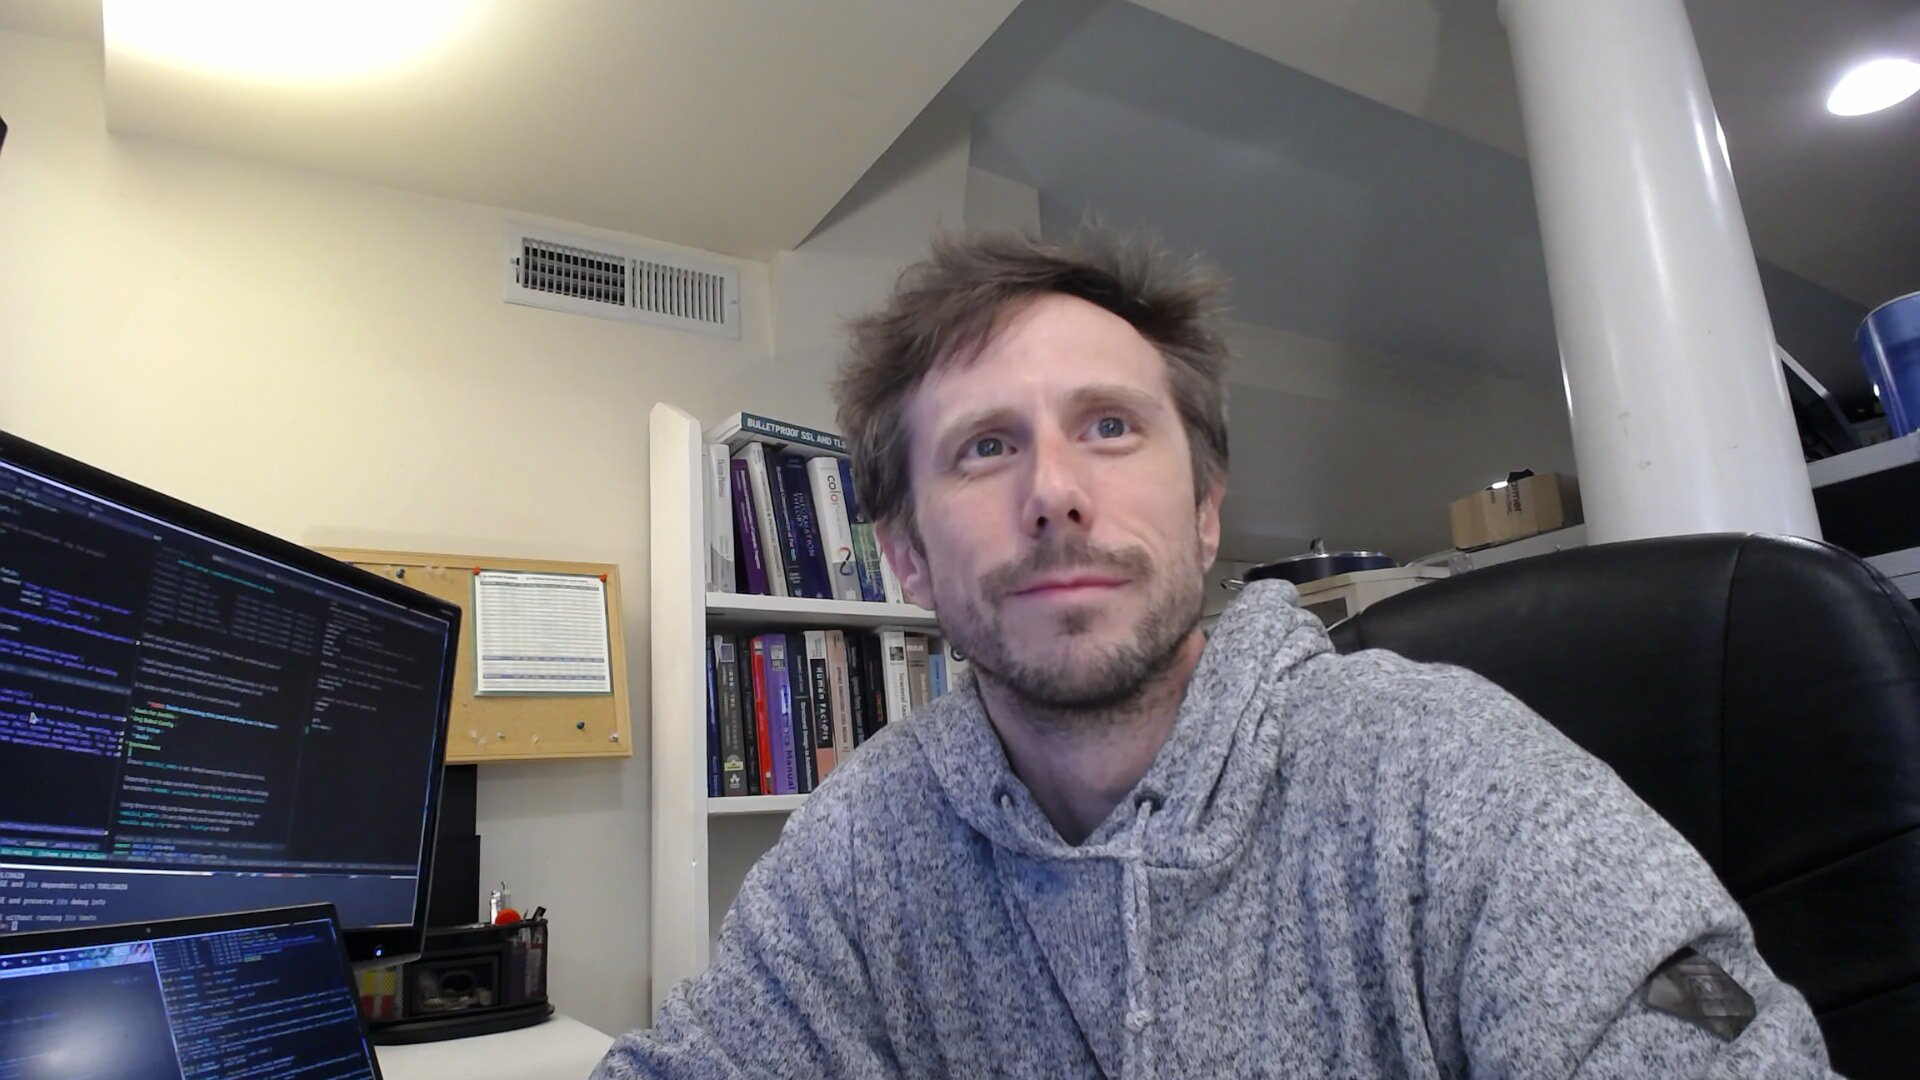
\includegraphics[width=1.2725\linewidth]{myphoto.jpg} %use full size
%---------------------------------------------------------------------------------------
%	QR CODE (optional)
%\vspace{-100pt}
%\hspace{0.59\linewidth}
%
\includegraphics[width=88pt]{qrcode}
%\normalsize
% \pareindent here is a hack
\setlength{\parindent}{5mm}

\vspace{-0.1cm}\\
\small{I'm an engineer with experience in networking, databases, containers,
and web applications. I'm looking to transition into a role that
leverages software to solve domain-specific problems, whether as an
application programmer or devops. I have experience integrating
disparate systems with minimal service interruptions and no loss of data.}

\small{I'm fast learner with a thirst for staying ahead in the technology world.
When practical, I prefer the source code as documentation for most tools.}\\[-2pt]
\textcolor{softcol}{\hrule}
\setlength{\parindent}{0mm}
\vspace{\spread}\\
\metasection{Hobbies:}{FOSS, Learning, Painting, Drawing, Kaggle, Electronics, Dance, Board Games, Writing}
\metasection{Apps:}{Blender, Krita, FreeCAD, OpenCascade, Inventor, Matlab, IRC}
\end{minipage}
\hfill
\begin{minipage}[t]{0.485\textwidth}


%---------------------------------------------------------------------------------------
%	SUMMARY (optional)
\vspace{\spread}

\cvsection{Summary}
\vspace{1pt}\\
\metasection{Lang:}{Bash, Ruby, Python, JS, TS, Clojure, Emacs Lisp, Scheme, Julia, Scala}
\metasection{Tools:}{Emacs, Org Mode, Direnv, Ansible, KDE, i3, VTY, GNU Screen, pyenv, poetry}
\metasection{Data:}{Reporting, ETL, Postgres, MSSQL, SQLite3, Parquet, jq}
\textcolor{softcol}{\hrule}
\vspace{\spread}\\
\metasection{Security:}{GPG, PIV, CA, Firewalls, Crypto}
\metasection{Linux:}{RPM, Guix, Docker, Podman, LVM}
\metasection{Cloud:}{Terraform, k8s, GCP}
\metasection{Homelab:}{SDN, VLAN, Proxmox, SR-IOV, UPS/Power}
\textcolor{softcol}{\hrule}
\vspace{\spread}\\
\setlength{\parindent}{5mm}
\small{\textbf{Interests:} Math, 3D Graphics, 3D Design, Philosophy, Futurism,
Writing, Linguistics, Semiotics, Bioinformatics, Epigenetics, Colorimetry,
Logistics, Materials}
\end{minipage}

\begin{minipage}[t]{0.485\textwidth}

\vspace{\spread}



%---------------------------------------------------------------------------------------
%	EDUCATION SECTION
\cvsection{Formal Education}\cvevent{2021 - 2023; 2006 - 2008}
{Mechatronics S.E.T.}
{Virginia Western Community College}
{\cvpoint{Obtained a Cisco CCNA certification (2008)} \\[2pt]
\cvpoint{Studied design, manufacture, electronics, CNC and safety}}
%
\cvrule{-8pt}{0pt}
%
\cvevent{2004 - 2006; 2008}
{Computer Science}
{Virginia Tech}
{\cvpoint{Studied Computer Science. Dropped out to compete in jamskating at a national level}}

%\textcolor{softcol}{\hrule}
\cvsection{Continuing Education}\cvevent{2012 -}
{Perennial Education}
{Coursera}
{\cvpoint{Certificates: Epigenetics, 2014; Bioinformatics I/II, 2015} \\[2pt]
\cvpoint{Other: Machine Learning, 2012; Drugs in the Brain, 2014}}
%
\cvrule{-8pt}{0pt}
%
\cvevent{2015 -}
{Perennial Education}
{Self-Directed Study}
{\cvpoint{Watched at least 1,000 hours of YouTube lectures on mathematics, engineering and emerging fields.} \\[2pt]
\cvpoint{Used the zettelkasten method to synthesize insights from dozens of fields.
Wrote essays combining cybernetics, semiotics, artificial intelligence, agency and sociology} \\[2pt]
\cvpoint{Designed a graphics library for Swift to leverage functional composition for dynamic rendering
pipelines using features unique to Metal}}
%
\cvrule{-8pt}{0pt}
%
\cvevent{2021 -}
{Automation}
{Homelab}
{\cvpoint{Developed ansible playbooks SDN for VLANS, Firewalls and IP Migration} \\[2pt]
\cvpoint{Created a Guix System image for GPG and Smallstep CA}}
%
\cvrule{-8pt}{0pt}
%
\cvevent{2021 -}
{Learning Craftsmanship For Independence}
{Workshop}
{\cvpoint{Modifying online designs to build a workbench and shelving} \\[2pt]
\cvpoint{Organized a workshop for woodworking, electronics, and making art supplies}}  % \\[\spread]

%\textcolor{softcol}{\hrule}

\end{minipage}
\hfill
\begin{minipage}[t]{0.485\textwidth}

\vspace{\spread}



%---------------------------------------------------------------------------------------
%	EXPERIENCE

\cvsection{Experience}\cvevent{2022 - 2023}
{Engineering Student Aide}
{Virginia Western Community College}
{\cvpoint{Maintained Ender-3 Pro and Raise3D printers. Synced Ender-3 configurations for PLA plastics} \\[2pt]
\cvpoint{Created an Autodesk Fusion CNC config for a Velocity CNC} \\[2pt]
\cvpoint{Collected notes on almost all equipment including support links and digital copies of manuals}} \\[\spread]
%
\cvrule{-8pt}{0pt}
%
\cvevent{2018}
{Cloud Engineer}
{RAKE Digital}
{\cvpoint{Used MS SQL table metadata to quickly learn the accounting database schema for Millennium and ReadyPay} \\[2pt]
\cvpoint{Designed an application stack with LoopbackJS and Angular 6 to automate payroll tasks in Azure}} % \\[\spread]
%
\cvrule{-8pt}{0pt}
%
\cvevent{2015 - 2017}
{Founder}
{Voxxel (Startup)}
{\cvpoint{Voxxel enabled fans to score their impersionations of movie quotes and accents} \\[2pt]
\cvpoint{Built a Rails API to back prototypes in iOS, Android and AngularJS. Each client processed and visualized the FFT}} % \\[\spread]
%
\cvrule{-8pt}{0pt}
%
\cvevent{2011 - 2015}
{Founder}
{Oscil8 (Startup)}
{\cvpoint{Oscil8 was designed to be the “Github for Music Producers”} \\[2pt]
\cvpoint{Developed a business model and strategic vision}}
%
\cvrule{-8pt}{0pt}
%
\cvevent{2014}
{Student Assistant / Programmer}
{Left + Right (Contract)}
{\cvpoint{Developed a web service to extend a Ruby on Rails application with reporting on SQL Views} \\[2pt]
\cvpoint{Cached report results in MongoDB to enable a dashboard}}
%
\cvrule{-8pt}{0pt}
%
\cvevent{2013}
{Student Assistant / Programmer}
{Jumpcloud}
{\cvpoint{Full stack development using a NodeJS API and MongoDB} \\[2pt]
\cvpoint{Integration tests using Mocha, Selenium and Soda}} % \\[\spread]

\end{minipage}


%	ARTIFICIAL FOOTER (fancy footer cannot exceed linewidth)

\null
\vspace*{\fill}
% this won't print
%\hspace{-0.25\linewidth}\colorbox{gray}{\makebox[1.5\linewidth][c]{\mystrut  \textcolor{bgcol}{www.jankuester.com $\cdot$ github.com/jankapunkt}}}
%\hspace{-0.25\linewidth}\colorbox{bgcol}{\makebox[1.5\linewidth][c]{\mystrut \textmd{\textcolor{white}{https://te.xel.io $\cdot$ github.com/dcunited001}}}}

\end{document}
